% !TEX root = base.tex
% --- Inserir folha de aprovação --- %

% Isto é um exemplo de Folha de aprovação, elemento obrigatório da NBR
% 14724/2011 (seção 4.2.1.3). Você pode utilizar este modelo até a aprovação
% do trabalho. Após isso, substitua todo o conteúdo deste arquivo por uma
% imagem da página assinada pela banca com o comando abaixo:

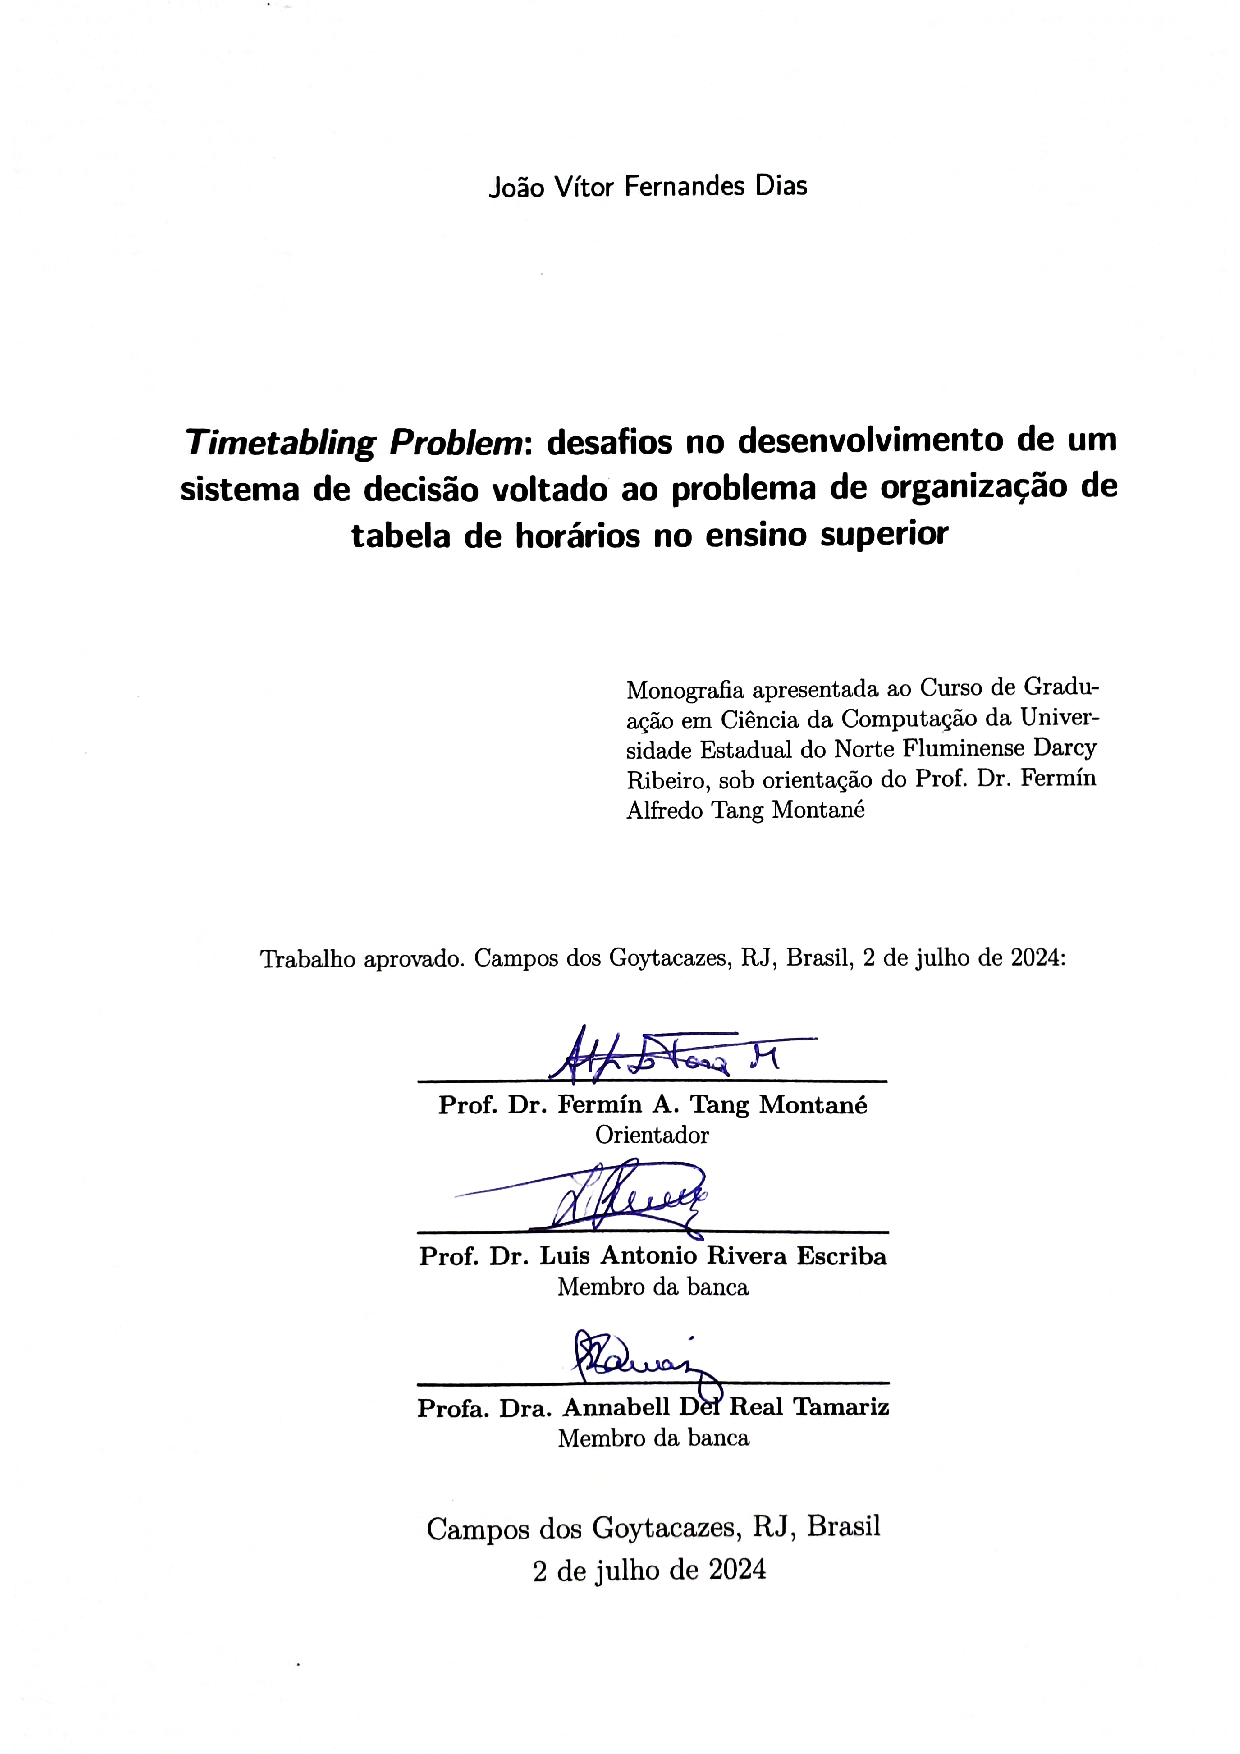
\includepdf{files/codigos/Folha de aprovação escaneada}

\begin{comment}

\begin{folhadeaprovacao}

  \begin{center}
    {\ABNTEXchapterfont\large\imprimirautor}

    \vspace*{\fill}\vspace*{\fill}
    \begin{center}
      \ABNTEXchapterfont\bfseries\Large\imprimirtitulo
    \end{center}
    \vspace*{\fill}

    \hspace{.45\textwidth}
    \begin{minipage}{.5\textwidth}
      \imprimirpreambulo
    \end{minipage}
    \vspace*{\fill}
  \end{center}

  Trabalho aprovado. \imprimirlocal, \DataImpressao :

  % \assinatura{\textbf{Prof. Dr. \imprimirorientador} \\ Orientador}
  \assinatura{\textbf{Prof. Dr. Fermín A. Tang Montané} \\ Orientador}
  \assinatura{\textbf{Prof. Dr. Luis Antonio Rivera Escriba} \\ Membro da banca}
  \assinatura{\textbf{Profa. Dra. Annabell Del Real Tamariz} \\ Membro da banca}
  %\assinatura{\textbf{Professor} \\ Convidado 3}
  %\assinatura{\textbf{Professor} \\ Convidado 4}

  \begin{center}
    \vspace*{0.5cm}
    {\large\imprimirlocal}
    \par
    {\large\DataImpressao}
    \vspace*{1cm}
  \end{center}

\end{folhadeaprovacao}
\end{comment}

% \chapter*{Banca}

% Por enquanto, a banca que eu tenho em mente é composta por:

% \begin{enumerate}
%   \item Fermín Alfredo Tang Montané (Orientador)
%   \item Annabell del Real Tamariz (Ex Chefe do Laboratório de Matemática)
%   \item Oscar Alfredo Paz La Torre (Ex Diretor do CCT)
%   \item Luiz Humberto Guillermo Felipe (Chefe do Laboratório de Matemática)
%   \item Márcia Diretora CCT (Diretora do CCT)
% \end{enumerate}

% Conforme resolução 004/2007 do COLAC, artigo 9 e parágrafo 1, a banca examinadora deverá ter a seguinte composição:
% (i) o Professor Orientador e/ou Co-orientador do aluno, que presidirá os trabalhos,
% (ii) um membro indicado, de comum acordo, pelo estudante e seu Professor Orientador ou Co-Orientador e
% (iii) um membro indicado pelo Colegiado do Curso. Em caráter excepcional, um dos três avaliadores poderá ser um Mestre ou doutorando ou pós doutorando que tenha formação compatível com o tema da monografia. Além dos membros titulares, deverá ser indicado um membro suplente. A composição da banca deverá ser aprovada pelo Colegiado do Curso, dando preferência para que o presidente seja doutor. Quando o orientador ou co-orientador estiver impossibilitado de estar presente na banca examinadora, o coordenador do Curso poderá representá-lo, desde que seja requerido por escrito e antecipadamente pelo orientador do aluno.
